\section*{Лекция 3}

Поговорим немного об облостях видимости.

\begin{minted}{cpp}
#include <iostream>

//глобальная область видимости

namespace N {
//область видимости namespace N
}

class C {
//область видимости класса C
};

int main() {
//область видимости функции
}
\end{minted}

Область видимости (\textbf{scope})~--- термин, который применяется к сущности 
и ограничивает ту часть программы, в которой эта сущность видна.

Если делать объявления в глобальной области видимости, то они будут видны отовсюду.

Началом scope будет являться открывающаяся фигурная скобка, концом~--- закрывающаяся.

Переменная, объявленная внутри scope функции называется \textbf{локальной}.
А если переменная объявлена в глобальном scope то она \textbf{глобальная}.

\begin{minted}{cpp}
#include <iostream>

int y;

int main() {
    int x;
}
\end{minted}

В данном случая переменная 'y' глобальная, а 'x'~--- локальная.

Можно создавать \textbf{безымянные} scope.

\begin{minted}{cpp}
#include <iostream>

int main() {
    int x;

    {
        int x;
    }
}
\end{minted}

Обратим внимание на то, что можно объявлять переменные с одинаковым именем в разных scope.

\begin{minted}{cpp}
#include <iostream>

int main() {
    int x = 4;

    {
        int x = 5;
        std::cout << x;
    }
    std::cout << x;
}
\end{minted}

По умолчанию действия применяются к ближайшей переменной по вложености к действию.

\begin{figure}[h]
    \centering
    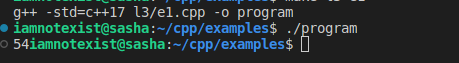
\includegraphics[width=0.8\textwidth]{l3img17.png}
    \caption{Обращение к переменным в разных scope 1.}
    \label{l3img17}
\end{figure}

Существует способ обращения к переменным из глобального scope.

\begin{minted}{cpp}
#include <iostream>

int x = 0;

int main() {
    int x = 4;
    std::cout << ::x;
    std::cout << x;
}
\end{minted}

\begin{figure}[h]
    \centering
    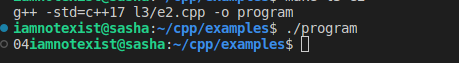
\includegraphics[width=0.8\textwidth]{l3img18.png}
    \caption{Обращение к переменным в разных scope 2.}
    \label{l3img18}
\end{figure}

Глобальная переменная 'x' \textbf{затмевается} локальной переменной 'x' в scope функции main.

\begin{minted}{cpp}
std::cout << ::x;
\end{minted}

Написав '::' перед переменной мы говорим что хотим использовать 'x' из глобального scope.


\begin{minted}{cpp}
#include <iostream>

namespace N {
    int x = 10;
}

int x = 5;

int main() {
    std::cout << N::x;
    std::cout << x;
}
\end{minted}

\begin{figure}[h]
    \centering
    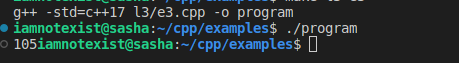
\includegraphics[width=0.8\textwidth]{l3img19.png}
    \caption{Обращение к переменным в разных scope 3.}
    \label{l3img19}
\end{figure}

Чтобы обратиться к переменной из scope namespace N нужно писать 'N::'.

Таким образом \textbf{std}~--- это namespace, объявленный в стандартной библиотеке.

\begin{minted}{cpp}
#include <iostream>

int main() {
    using namespace std;

    int x = 5;
    std::cout << x;
}
\end{minted}

\begin{figure}[h]
    \centering
    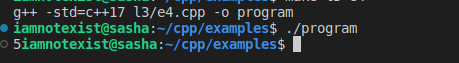
\includegraphics[width=0.8\textwidth]{l3img20.png}
    \caption{Вливание std.}
    \label{l3img20}
\end{figure}

Написав using namespace std мы сливаем namespace std со скоупом функции main и можем обращаться к cout без префикса std::.

Делать подобное не рекомендуется поскольку std довольно большой и велик риск коллизии объявлений.

Влить в scope функции можно и что-то конкретное.

\begin{minted}{cpp}
using std::cout;
\end{minted}

В C++ есть некоторые понятия. Если переменная используется без префикса scope, то это
\textbf{unqulified-id}, а если с префиксом то это \textbf{qulified-id}.

\subsection{Basic types and supported operation.}

C++~--- статически типизированный язык. Это значит, что у каждой переменной должен быть тип 
и он должен быть известен на этапе компиляции.

У переменной нельзя менять ее тип.

Приведем примеры базовых целочисленных типов:
\begin{itemize}
    \item short - обычно 2 байта, [-2**15; 2**15)
    \item int - обычно 4 байта, [-2**31; 2**31)
    \item long - обычно 4 байта, [-2**31; 2**31)
    \item long long - обычно 8 байт, [-2**63; 2**63)
\end{itemize}

Помимо этого у них есть беззнаковые версии:
\begin{itemize}
    \item unsigned short - обычно 2 байта, [0; 2**16)
    \item unsigned int - обычно 4 байта, [0; 2**32)
    \item unsigned long - обычно 4 байта, [0; 2**32)
    \item unsigned long long - обычно 8 байт, [0; 2**64)
\end{itemize}

Также в прогрмме можно написать просто unsigned. По умолчанию будет считаться, что это unsigned int.
Размер этих типов не определен стандартом. Однако иногда требуется точность, поэтому существуют следущие типы.

\begin{itemize}
    \item int16\_t -  2 байта, [-2**15; 2**15)
    \item int32\_t -  4 байта, [-2**31; 2**31)
    \item int64\_t -  8 байт, [-2**63; 2**63)
    \item uint16\_t - 2 байта, [0; 2**16)
    \item uint32\_t - 4 байта, [0; 2**32)
    \item uint64\_t - 8 байт, [0; 2**64)
\end{itemize}

Существует также тип \textbf{size\_t}, который является alias для некоторого беззнакового типа.
То какого типа это alias зависит от размера адресного пространства.

Перейдем к вещественным типам.

\begin{itemize}
    \item float - обычно 4 байта
    \item double - обычно 8 байт
    \item long double - обычно 16 байт
\end{itemize}

Рассмотрим по подробнее double.

\begin{figure}[h]
    \centering
    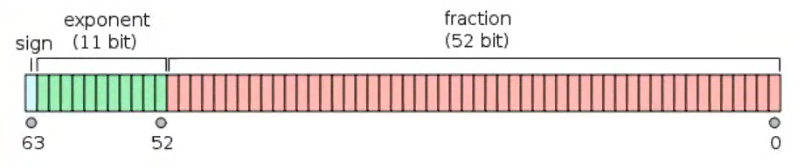
\includegraphics[width=1.2\textwidth]{l3img21.png}
    \caption{Представление double.}
    \label{l3img21}
\end{figure}

1 старший бит отводится под знак. 11 бит под экспоненту.
52 бита под мантиссу.

В экспоненте записано число~--- степень, в которую нужно возвести двойку.
В мантиссе информация о втором множителе.